%
%===============>>  Ленотьева Модуль 7 <<=============
%
\setmodule{7}

%BEGIN_FOLD % ====>>_____ Занятие 1 _____<<====
\begin{class}[number=1]
	\begin{listofex}
		\item Занятие 1
	\end{listofex}
\end{class}
%END_FOLD

%BEGIN_FOLD % ====>>_____ Занятие 2 _____<<====
\begin{class}[number=2]
	\begin{listofex}
		\item На рисунке изображён график функции \( y=f(x) \) левая круглая скобка x правая круглая скобка . Какие из утверждений относительно этой функции неверны? Укажите их номера.
		\begin{figure}[h!]
			\centering
			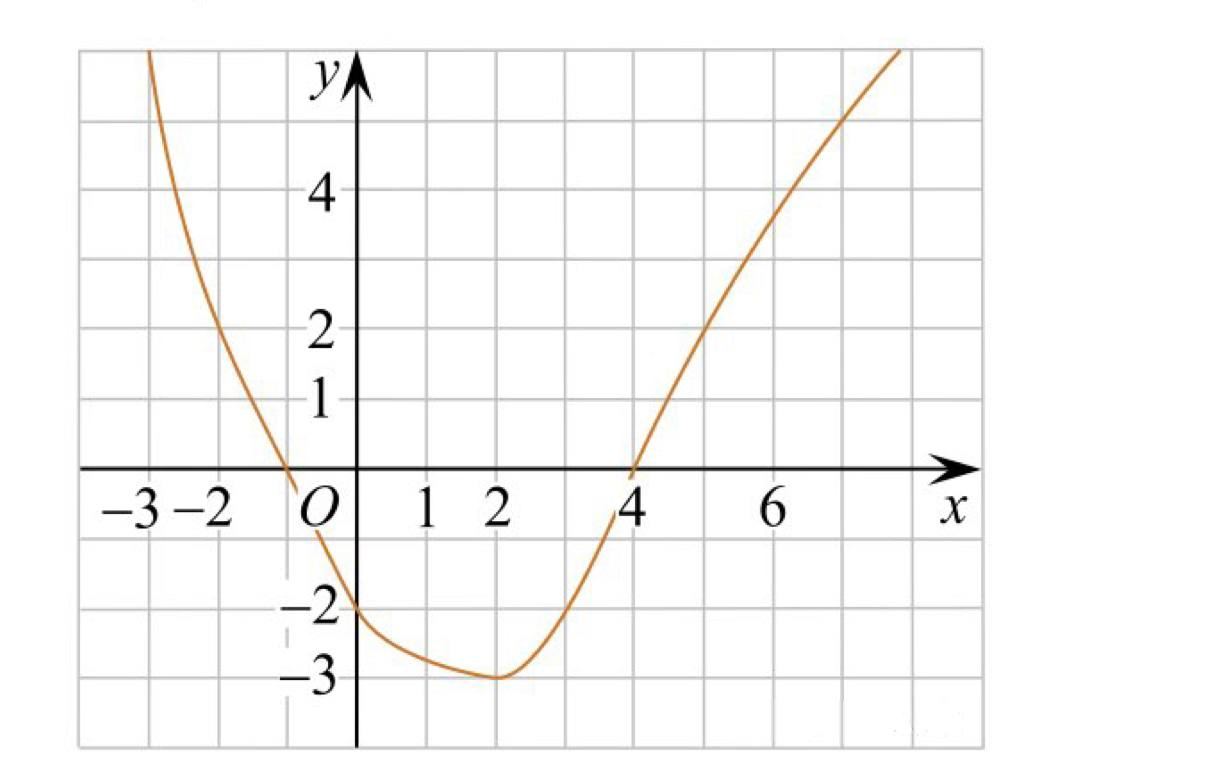
\includegraphics[width=0.4\linewidth]{../../../../../exercises/lists/pics/leontevaM7L2-1}
		\end{figure}
		\begin{tasks}(1)
			\task функция возрастает на промежутке  \( [-2; +\infty) \)
			\task \( f(3)> f(-3)  \)
			\task \( f(0) = -2 \)
			\task прямая y=2  пересекает график в точках \(  (-2; 2) \)  и \( (5; 2) \) 
		\end{tasks}
		\item На рисунке изображён график квадратичной функции \( y  =  f(x) \).
		\\
		Какие из следующих утверждений о данной функции неверны? Запишите их номера в порядке возрастания.
		\begin{figure}[h!]
			\centering
			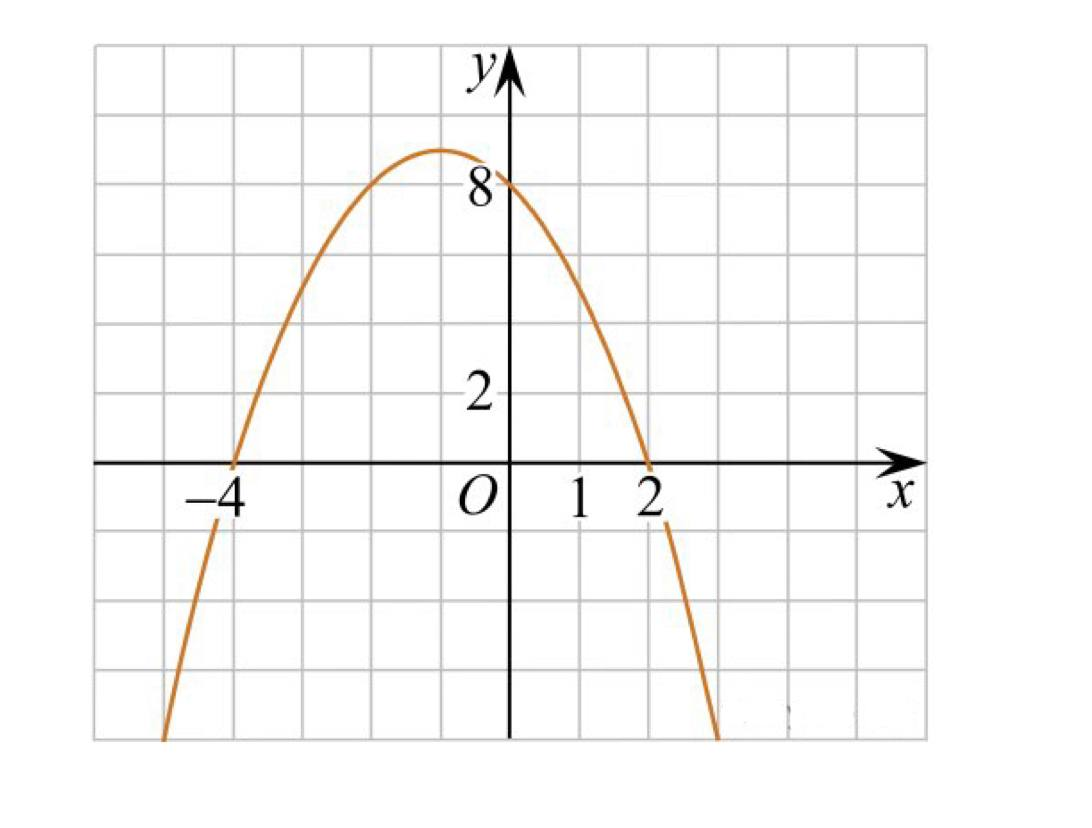
\includegraphics[width=0.4\linewidth]{../../../../../exercises/lists/pics/leontevaM7L2-2}
		\end{figure}
		\begin{tasks}(1)
			\task Функция возрастает на промежутке \( (-\infty;  -1 \)].
			\task Наибольшее значение функции равно \( 8 \).
			\task \( f(-4) \neq f(2) \).
		\end{tasks}
		\newpage
		\item На рисунке изображён график квадратичной функции \( y =  f(x) \).
		Какие из следующих утверждений о данной функции неверны? Запишите их номера.
		\begin{figure}[h!]
			\centering
			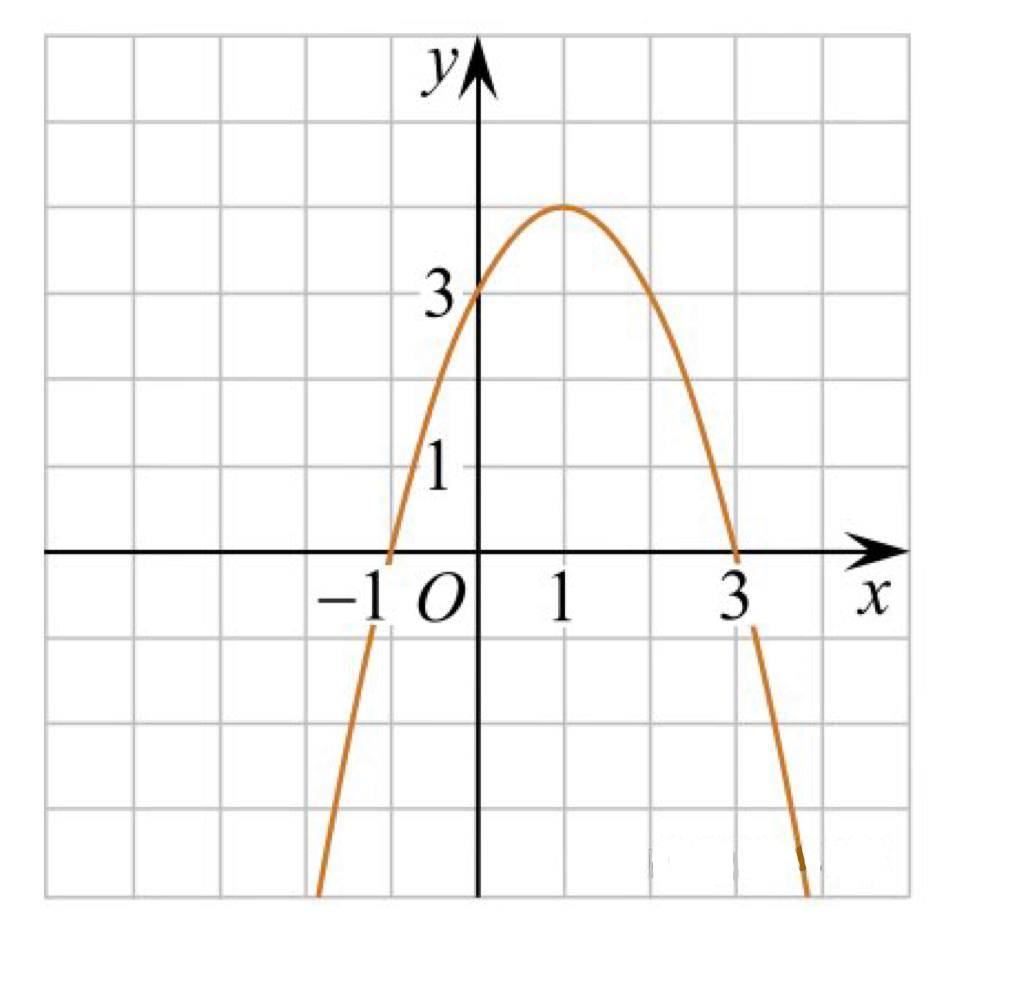
\includegraphics[width=0.4\linewidth]{../../../../../exercises/lists/pics/leontevaM7L2-3}
		\end{figure}
		\begin{tasks}(1)
			\task \( f(-1)=f(3) \).
			\task Наибольшее значение функции равно \( 3 \).
			\task \( f(x)>0  \) при  \( -1<x<3 \).
		\end{tasks}
		\item На рисунке изображён график квадратичной функции \( y = f(x) \).
		
		Какие из следующих утверждений о данной функции неверны? Запишите их номера.
		\begin{figure}[h!]
			\centering
			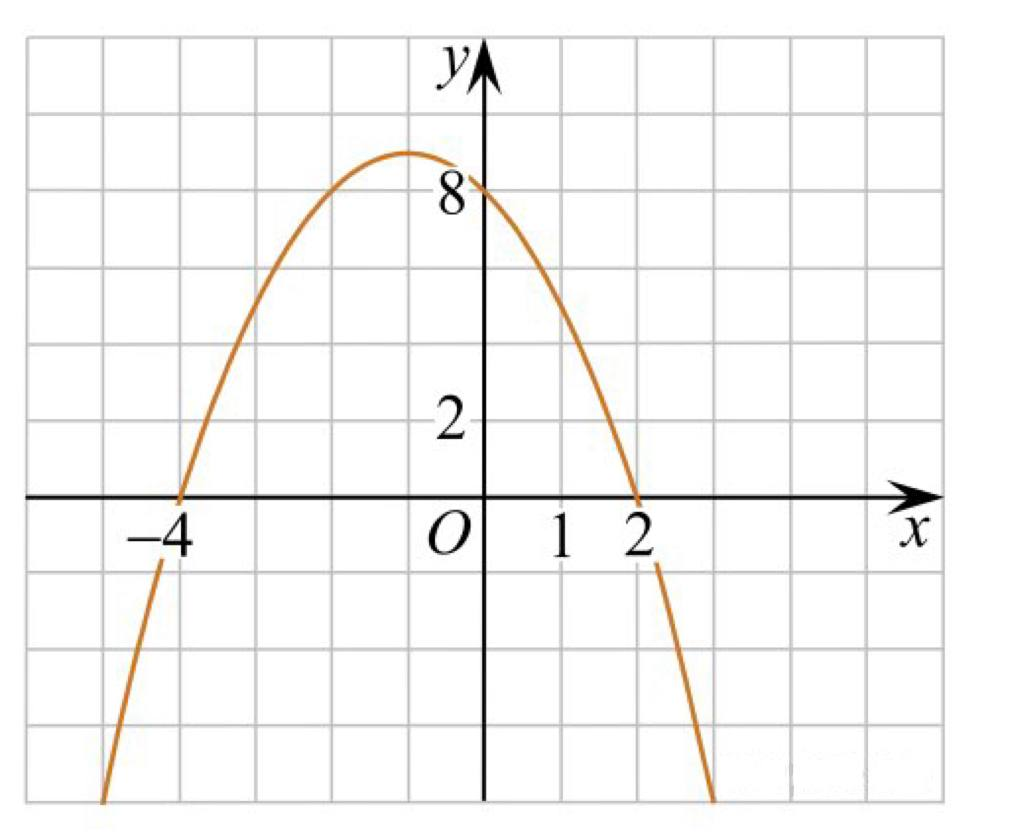
\includegraphics[width=0.4\linewidth]{../../../../../exercises/lists/pics/leontevaM7L2-4}
		\end{figure}
		\begin{tasks}(1)
			\task  Наибольшее значение функции равно \( 9 \).
			\task \( f(0)>f(1) \).
			\task \( f( x )>0 \) при \( x<0 \).
		\end{tasks}
		\newpage
		\item На рисунке изображён график функции \(  y = ax2 + bx + c \). Установите соответствие между утверждениями и промежутками, на которых эти утверждения выполняются. 
		\begin{figure}[h!]
			\centering
			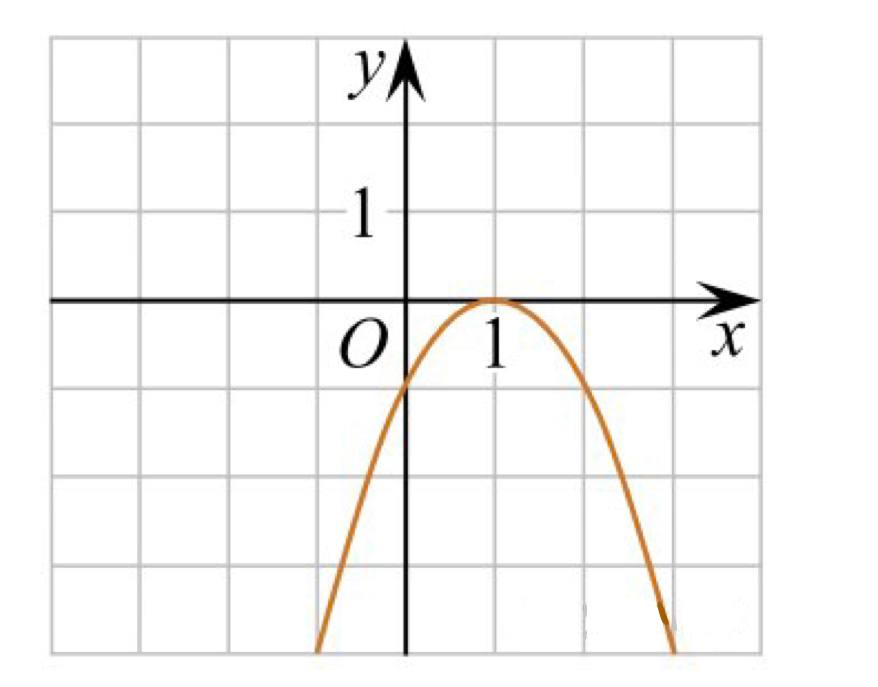
\includegraphics[width=0.3\linewidth]{../../../../../exercises/lists/pics/leontevaM7L2-5}
		\end{figure}
		\begin{tasks}(2)
			\task[] УТВЕРЖДЕНИЯ	 
			\task[]	ПРОМЕЖУТКИ
			\task[A)] функция возрастает на промежутке
			\task \( [1;2] \)
			\task[B)]функция убывает на промежутке
			\task \( [0;2] \)
			\task[]
			\task\( [-1;0] \)
			\task[]
			\task\( [-2;3] \)
		\end{tasks}
		\item 
		На рисунке изображён график функции \(  y = ax2 + bx + c \). Установите соответствие между утверждениями и промежутками, на которых эти утверждения выполняются. 
		\begin{figure}[h!]
			\centering
			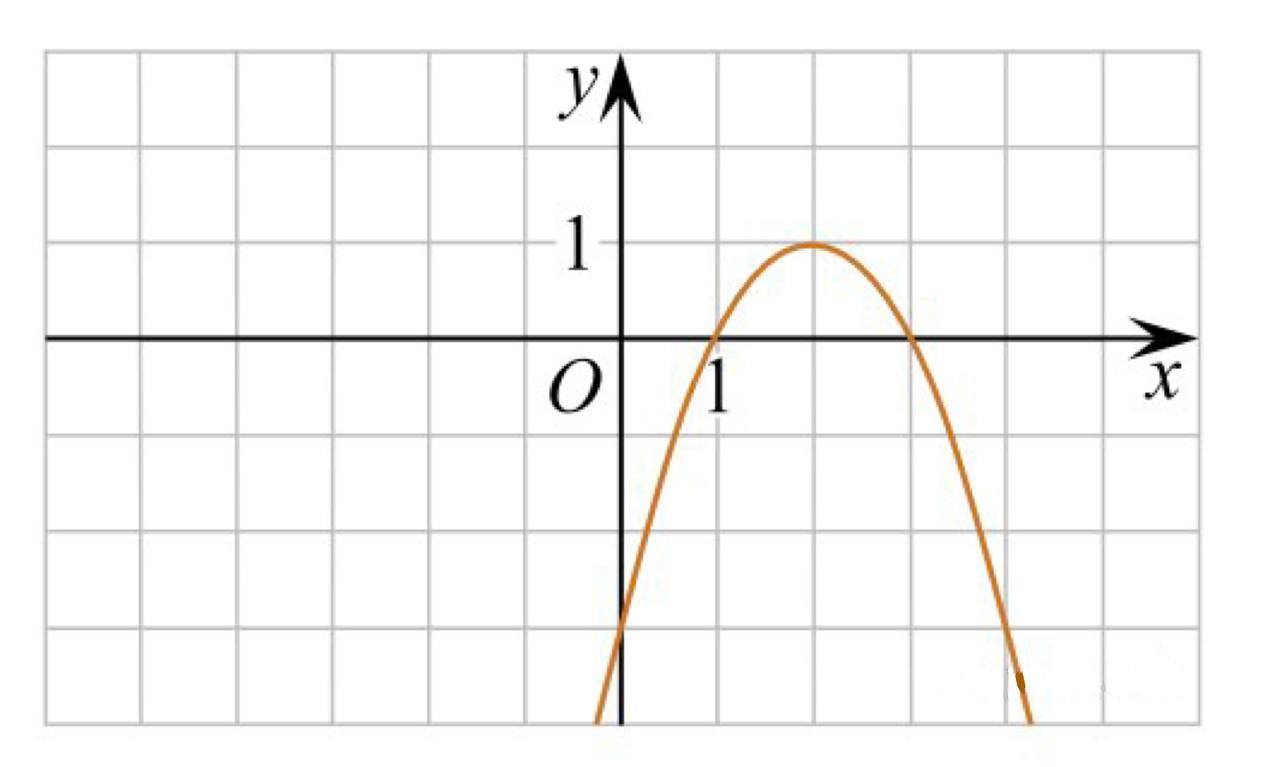
\includegraphics[width=0.3\linewidth]{../../../../../exercises/lists/pics/leontevaM7L2-6}
		\end{figure}
		\begin{tasks}(2)
			\task[] УТВЕРЖДЕНИЯ	 
			\task[]	ПРОМЕЖУТКИ
			\task[A)] функция возрастает на промежутке
			\task \( [0; 3] \)
			\task[B)]функция убывает на промежутке
			\task \( [-1; 1] \)
			\task[]
			\task\( [2; 4] \)
			\task[]
			\task\( [1; 4] \)
		\end{tasks}
		\item Найдите координаты вершины параболы \( y = 2x^{2} + 4x + 5 \).
		\item Найдите координаты вершины параболы\(  y = -x^{2} + 2x - 4 \).
		\item Найдите координаты вершины параболы\(  y = \dfrac{1}{3}x^{2}+x-1 \).
		\item Найти вершину параболы, заданной формулой \( y=2x^{2} - 8x + 5. \)
	\end{listofex}
\end{class}
%END_FOLD

%BEGIN_FOLD % ====>>_____ Занятие 3 _____<<====
\begin{class}[number=3]
	\begin{listofex}
		\item Один из смежных углов на \( 40^{\circ} \) больше другого. Найдите эти углы.
		\item Внутри развернутого угла \( PNE \) провели луч  \( NR \). Найди каждый из двух  образовавшихся углов, если один из них в \( 4 \) раза больше другого.  
		\item При пересечении двух прямых образовались такие углы, что сумма двух из них равна \( 100^{\circ} \). Найди все углы.
		\item В треугольнике \( ABC \)    \( AB=BC \),   внешний угол при вершине \( B  \)  равен \( 138^{\circ} \).   Найдите \( \angle C \).   Ответ дайте в градусах.
		\item В треугольнике \( ABC \)   \( \angle B= 39^{\circ} \) ,  \(  AB  =BC \).   Найдите внешний угол при вершине \( A \).   Ответ дайте в градусах.
		\item В равнобедренном треугольнике \( ABC \)  внешний угол при вершине \( B \) равен \( 86^{\circ} \). Найдите наименьший из внутренних углов этого треугольника. Ответ дайте в градусах.
		\item В треугольнике \( ABC \)  \( \angle A = 52^{\circ} \), \( \angle C = 71^{\circ} \).На продолжении стороны \( BC \)   за точку \( B \)   отложен отрезок \( BD = AB \).   Найдите \( \angle D \)   треугольника \( ABD \).   Ответ дайте в градусах.
		\item В треугольнике \( ABC \)   \( \angle A = 22^{\circ} \),   внешний угол при вершине \( C \)   равен \( 130^{\circ} \).   Найдите \( \angle B \).   Ответ дайте в градусах.
		\item Найдите углы треугольника, зная, что внешние углы при двух его вершинах равны \( 130^{\circ} \) и \( 140^{\circ} \).
		\item Один из углов, образовавшихся при пересечении двух прямых, равен \( 45^{\circ} \). Найди остальные углы.
		\item Биссектрисы углов \( N \) и \( M \) треугольника \(  MNP \) пересекаются в точке \( A \). Найдите \( \angle NAM \), если \( \angle N=84^{\circ} \), а \( \angle M=42\degree \). 
		\item Углы треугольника относятся как \(  2:8:35 \). Найдите меньший из них. Ответ дайте в градусах.
		\item Два угла треугольника равны \( 58^{\circ} \) и \( 72^{\circ} \). Найдите тупой угол, который образуют высоты треугольника, выходящие из вершин этих углов. Ответ дайте в градусах.
		\item В треугольнике \( ABC \) \( CH \)  — высота, \( AD \)  — биссектриса, \( O \) — точка пересечения прямых \( CH \) и \( AD \),  \( \angle BAD \) равен \( 26^{\circ} \). Найдите \( \angle AOC \). Ответ дайте в градусах.
	\end{listofex}
\end{class}
%END_FOLD

%BEGIN_FOLD % ====>>_____ Занятие 4 _____<<====
\begin{class}[number=4]
	\begin{listofex}
		\item Один из острых углов прямоугольного треугольника на \( 24^{\circ} \) больше другого. Найдите углы данного треугольника. Ответ дайте в градусах.
		\item В треугольнике \( ABC \): \( C=90^{\circ} \), \( AB=8 \) и \( BC=5 \). Найдите \( AC \).
		\item Дан прямоугольный треугольник \( ABC \), \( \angle C=90^{\circ} \), и \( AC=3 \), \( BC=4 \). Найдите длину \( AB \).
		\item Два острых угла прямоугольного треугольника относятся как \( 4:5 \). Найдите больший острый угол. Ответ дайте в градусах.
		\item В прямоугольном треугольнике катет и гипотенуза равны \( 40 \) и \( 41 \) соответственно. Найдите другой катет этого треугольника.
		\item Катеты прямоугольного треугольника равны \( 8 \) и \( 15 \). Найдите гипотенузу этого треугольника.
		\item Катеты прямоугольного треугольника равны \( 18 \) и \( 24 \). Найдите высоту, проведенную к гипотенузе.
		\item В треугольнике \( ABC \) угол \( C \) равен \( 90^{\circ} \), \( M \)  — середина стороны \( AB \), \( AB  =  20 \), \( BC = 10 \). Найдите \( CM \).
		\item Биссектриса равностороннего треугольника равна  \( 4\sqrt{3} \). Найдите сторону этого треугольника.
		\item Диагонали ромба равны \( 14 \) см и \( 48 \) см. Найдите сторону ромба.
		\item В треугольнике два угла равны \( 45\degree \) и \( 90\degree \), а большая сторона — \( 20 \) см. Найдите две другие стороны треугольника и запишите их сумму .
		\item Стороны прямоугольника равны \( 8 \) см и \( 12 \) см. Найдите его диагональ.
	\end{listofex}
\end{class}
%END_FOLD

%BEGIN_FOLD % ====>>_ Домашняя работа 2 _<<====
\begin{homework}[number=2]
	\begin{listofex}
		\item Домашняя работа 2
	\end{listofex}
\end{homework}
%END_FOLD

%BEGIN_FOLD % ====>>_____ Занятие 5 _____<<====
\begin{class}[number=5]
	\begin{listofex}
		\item Занятие 5
	\end{listofex}
\end{class}
%END_FOLD

%BEGIN_FOLD % ====>>_____ Занятие 6 _____<<====
\begin{class}[number=6]
	\begin{listofex}
		\item Занятие 6
	\end{listofex}
\end{class}
%END_FOLD

%BEGIN_FOLD % ====>>_ Домашняя работа 3 _<<====
\begin{homework}[number=3]
	\begin{listofex}
		\item Домашняя работа 3
	\end{listofex}
\end{homework}
%END_FOLD

%BEGIN_FOLD % ====>>_____ Занятие 7 _____<<====
\begin{class}[number=7]
	\title{Подготовка к проверочной}
	\begin{listofex}
		\item Занятие 7
	\end{listofex}
\end{class}
%END_FOLD

%BEGIN_FOLD % ====>>_ Проверочная работа _<<====
\begin{exam}
	\begin{listofex}
		\item Проверочная
	\end{listofex}
\end{exam}
%END_FOLD